\section{Theorem-aligned synthetic experiments}
\label{sec:experiments}

The experiments test the mathematical mechanisms before an expensive LLM study. They do not establish a practical improvement on open models. Code, seeds, and full CSV files accompany the paper.

\subsection{TT tangent dimension and the \texorpdfstring{\(d/(2n)\)}{d/(2n)} law}

We generated generic order-four TT tensors with mode sizes \((4,4,4,4)\) and uniform internal ranks \(r=1,2,3\). A finite-difference Jacobian mapped raw core perturbations to the contracted ambient tensor. We compared its numerical rank with the gauge-adjusted formula, and the left singular vectors spanning its image formed an orthonormal horizontal tangent.

For a tangent of dimension \(d\), Gaussian prompts induced tangent design \(A\sim N(0,I_d)\). The frozen base tensor supplied an offset \(b(X)\), the teacher returned
\(Y\sim\operatorname{Bernoulli}\{\operatorname{logit}^{-1}(b)\}\), and the local student had logit \(b+A^\top\theta\). We fitted \(\theta\) by likelihood and evaluated exact Bernoulli KL on 12,000 new prompts. Each condition used 80 Monte Carlo replications.

\Cref{tab:geometry,fig:tt-rate} report the quotient-dimension check and the
corresponding population-KL rate experiment.

\begin{table}[t]
\centering
\caption{The contraction Jacobian removes exactly the TT gauge directions.}
\label{tab:geometry}
\begin{tabular}{rrrrr}
\toprule
TT rank & Raw cores & Gauge & Formula \(d_{TT}\) & Jacobian rank\\
\midrule
1 & 16 & 3 & 13 & 13\\
2 & 48 & 12 & 36 & 36\\
3 & 96 & 27 & 69 & 69\\
\bottomrule
\end{tabular}
\end{table}

\begin{figure}[t]
\centering
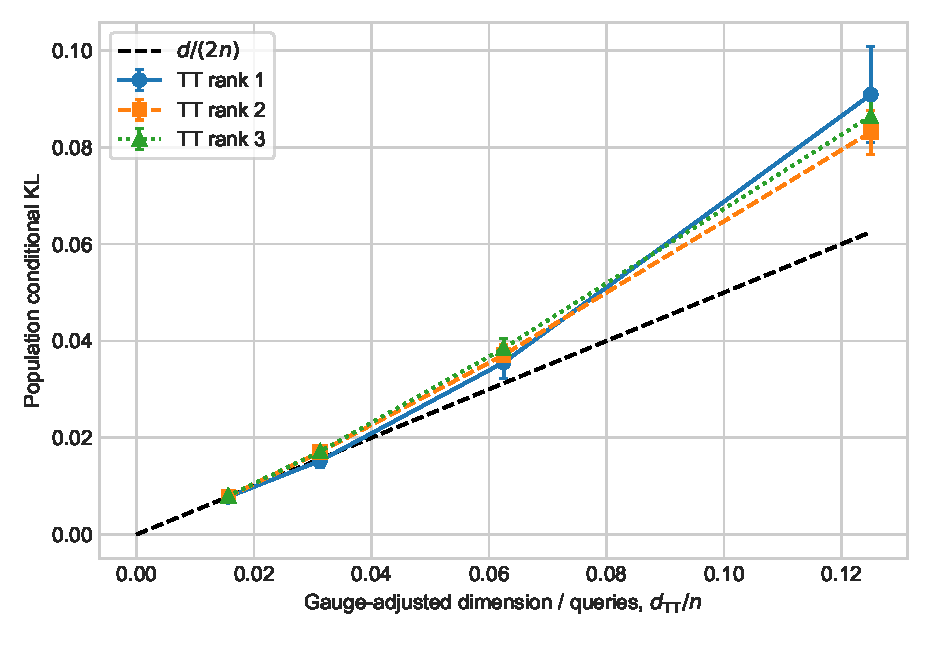
\includegraphics[width=.72\textwidth]{../figures/tt_rate.pdf}
\caption{Risks from all three TT ranks collapse when indexed by \(d_{TT}/n\). The black dashed line is the local asymptotic prediction \(d_{TT}/(2n)\); bars are pointwise 95\% Monte Carlo intervals, and marker/line shape identifies TT rank.}
\label{fig:tt-rate}
\end{figure}

Table~\ref{tab:geometry} verifies the quotient count exactly. At \(n/d=64\), the values of \(n\wh\cD/d\) are 0.497, 0.502, and 0.510 for ranks 1, 2, and 3. The average over all twelve conditions is 0.579; the excess above one half is concentrated in the smaller \(n/d\) conditions, as expected from finite-sample likelihood curvature. Figure~\ref{fig:tt-rate} shows that data from all three raw core counts collapse when indexed by the quotient dimension.

\subsection{Access-regime counterexample}

We next used \(d=20\). In the black-box experiment, the teacher was Bernoulli(1/2) and one response was sampled per prompt. In the exact-soft-label experiment, the value 1/2 was supplied as a fractional label. A misspecified soft-label condition used the nonlinear teacher
\[
q_0(1\mid X)=\operatorname{logit}^{-1}\left[
0.65\{\norm{X}^2-d\}/\sqrt{2d}\right]
\]
and a linear-logit student. Symmetry made the population projection zero, while prompt-specific gradients remained random.

\Cref{fig:access} compares the population excess risks under these three
observation regimes.

\begin{figure}[t]
\centering
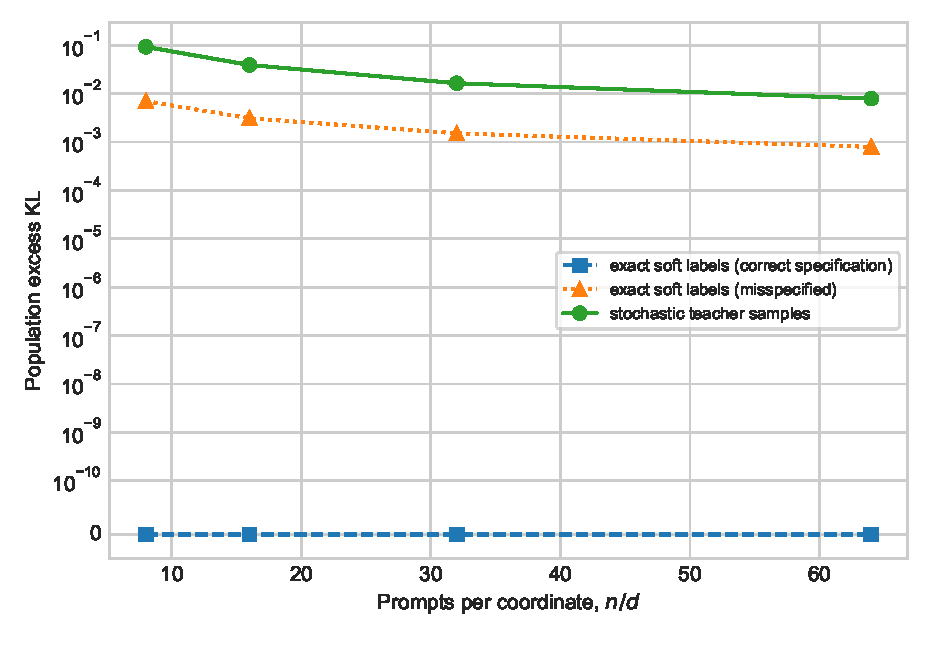
\includegraphics[width=.72\textwidth]{../figures/access_regimes.pdf}
\caption{The black-box risk decays at the usual parametric rate.  In this identifiable logistic example, exact soft labels recover the correctly specified parameter with zero numerical estimation error; the misspecified case has a smaller prompt-quadrature-dependent \(1/n\) term. The vertical scale is symmetric-log to display the exact zeros.}
\label{fig:access}
\end{figure}

With \(n/d=64\), \(n\wh\cD/d\) is 0.504 for stochastic responses, exactly zero to numerical precision for correctly specified soft labels, and 0.051 for misspecified soft labels. This instantiates the counterexample in \cref{prop:access}; it does not assert zero risk for every soft-label model. Under misspecification, the coefficient is determined by prompt-gradient variance rather than dimension alone.

\subsection{Functional misordering and a Gaussian benchmark}

For the explicit construction in \cref{prop:tt-misordering-paths}, we used the orthonormal rank-one TT atoms \(T_H=e_0^{\otimes4}\) and \(T_L=e_1^{\otimes4}\), amplitudes \(a=0.8\), \(b=1\), and scale \(t=0.5\). Both students have TT rank one and identical storage. Their Frobenius errors are 0.4 and 0.5, so reconstruction always selects \(A\). We then evaluated the exact Bernoulli KL, rather than substituting its quadratic expansion. As \(\rho_H/\rho_L\) ranges from 2 to 32, functional selection reduces exact population risk by factors 1.294 to 20.707; see \cref{fig:misordering-oracle}(a). The quadratic prediction, shown separately, is already close at this finite scale.

Finally, a separate Gaussian horizontal-coordinate experiment used candidate dimensions \(13,36,69,112\), the quotient dimensions of uniform-rank order-four TT models, and a polynomially decaying teacher. Mallows' unbiased criterion selected a truncation on the same observations. Over 3,000 replications, mean selected risk was between 1.023 and 1.102 times the infeasible minimum of approximation error plus \(d/n\); see \cref{fig:misordering-oracle}(b). This experiment illustrates the Gaussian-sequence benchmark in \cref{cor:scale}; because it fits neither TT cores nor a conditional generator, it does not validate the conditional-generator oracle in \cref{thm:oracle}.

\begin{figure}[t]
\centering
\begin{subfigure}{.48\textwidth}
\centering
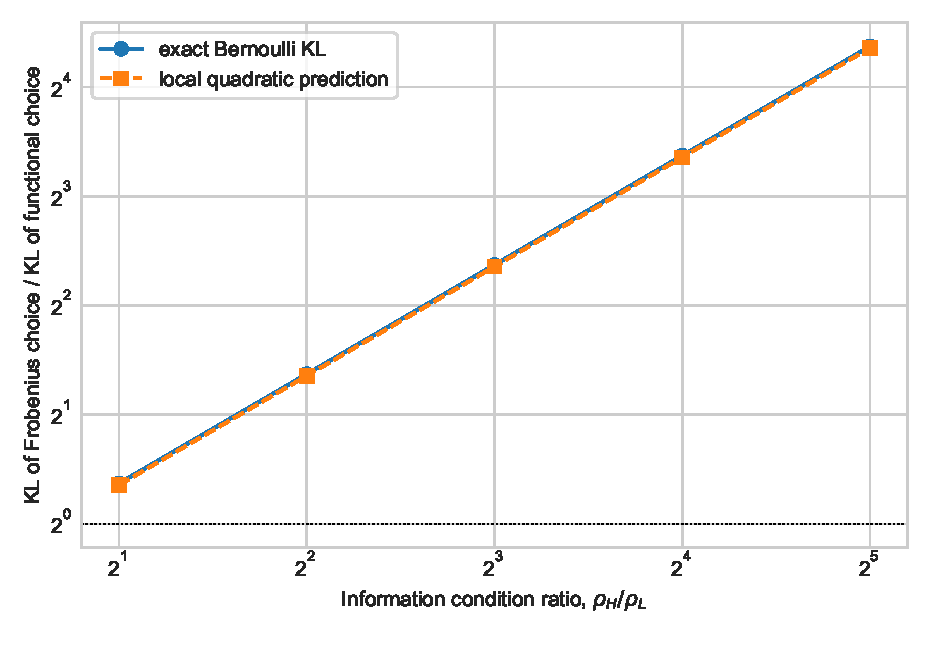
\includegraphics[width=\textwidth]{../figures/metric_misordering.pdf}
\caption{Metric misordering.}
\end{subfigure}\hfill
\begin{subfigure}{.48\textwidth}
\centering
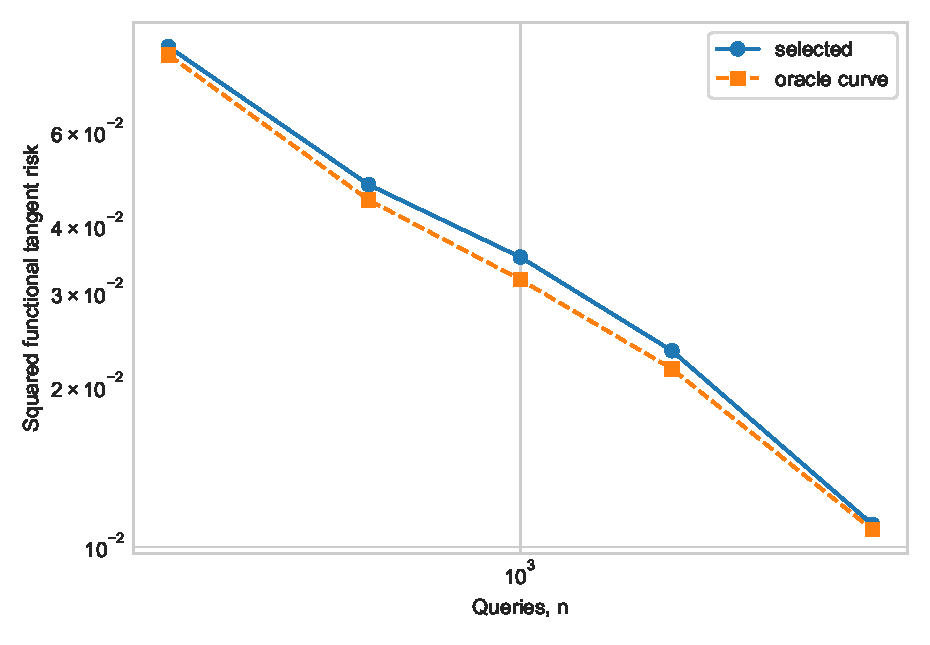
\includegraphics[width=\textwidth]{../figures/oracle_adaptation.pdf}
\caption{Gaussian selected versus benchmark risk.}
\end{subfigure}
\caption{Functional selection avoids a risk ratio that grows with metric anisotropy, while penalized coordinate selection stays close to its separate Gaussian-sequence benchmark. Panel (a) evaluates exact Bernoulli KL for two equal-budget rank-one TT students and overlays the local quadratic prediction; panel (b) averages 3,000 Gaussian-sequence replications at each \(n\) and is not a conditional-generator experiment.}
\label{fig:misordering-oracle}
\end{figure}

\subsection{Preregistered empirical falsification gate}

A subsequent open-model study should compare functional conditional-KL or Jacobian-pullback allocation against Frobenius, spectral, activation-reconstruction, and current loss-aware rank allocation on at least two model families. Ranks must be learned on calibration prompts and evaluated on held-out distributions and multiple capabilities. The theory-first direction should be abandoned or reframed if: (i) functional criteria do not improve held-out allocation ordering; (ii) the estimated functional information is effectively low rank and unstable across prompt resamples; or (iii) attainable optimizers cannot approach the oracle curve in a tractable frozen nonlinear block. This gate prevents the synthetic rate verification from being presented as evidence of LLM-scale benefit.
